\chapter{Ejercicios extra criptografía}


\section{Ejercicio 1:}


\begin{lstlisting}
# En este ejercicio se intenta por fuerza bruta encontrar tanto x como y:

x = 1
break_p <- FALSE

while(!break_p){
  if(3^x %% 47 == 28){
    break_p <- TRUE
    print(x)
  }else{
    x <- x + 1 
  }
}

y = 1
break_p <- FALSE

while(!break_p){
  if(3^y %% 47 == 17){
    break_p <- TRUE
    print(y)
  }else{
    y <- y + 1 
  }
}

\end{lstlisting}

De esta forma, x y y son 8 y 10 respectivamente



\begin{figure}[!h]
        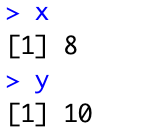
\includegraphics[width=15mm]{imgs/Captura de Pantalla 2021-02-13 a la(s) 14.30.24.png}
\end{figure}

\newpage 


\section{Ejercicio 2:}

\begin{lstlisting}
# Esta libreria nos permite transformar un numero entero a su equivalente binario
library(binaryLogic)

# La function 'construir_vector_base' permite calcular los residuos de base^1, base^2, base^4, base^8 y base^16 o hasta el binario necesario modulo 'mod'. 

construir_vector_base <- function(bin, mod, base){
  residuo <- c()
  
  # Inicializamos el vector residuo con base^1 modulo mod
  inicial <- base^1 %% mod
  residuo <- c(inicial)
  
  # Llenamos el vector de residuos con los demas residuos de base^i. Para esto utilizamos los elementos anteriores de residuo para evitar computo extra
  for(i in 2:length(bin)){
    num_ant <- (residuo[length(residuo)])
    residuo <- c(residuo, (num_ant*num_ant) %% mod)
  }
  
  # regresamos el vector residuo
  return(residuo)
}


# obtener residuo nos ayuda a transformar el numero deseado a binario, calcular su vector de residuos y calcular el modulo del numero original 
obtener_residuo <- function(exp, mod, base){
  
  bin <- rev(as.binary(exp))
  residuos <- construir_vector_base(bin, mod, base)  
  vec_nums <- as.numeric(as.character(bin)) * residuos
  prod(vec_nums[vec_nums>0]) %% mod
  
}

# ejemplo (resultado = 12):
obtener_residuo(29, 35, 17)

\end{lstlisting}

\begin{figure}[!h]
        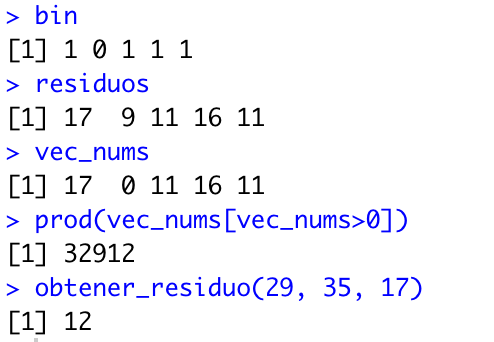
\includegraphics[width=45mm]{imgs/Captura de Pantalla 2021-02-13 a la(s) 14.44.58.png}
\end{figure}

